% \documentclass[handout]{beamer}
\documentclass[presentation]{beamer}
\usepackage[utf8]{inputenc}
\usepackage{amsmath, pdfpages, pdflscape, lscape, color, listings, hyperref, amssymb, graphicx, textcomp,varioref, afterpage, subcaption, float, bm, tikz, colortbl}

\global
\newcommand{\Fig}[1]{Figure \ref{#1}}
\newcommand{\fig}[1]{figure \ref{#1}}
\newcommand{\tab}[1]{table \ref{#1}}
\newcommand{\eq}[1]{equation \ref{#1}}
\newcommand{\Eq}[1]{Equation \ref{#1}}
\newcommand{\alg}[1]{algorithm \ref{#1}}
\newcommand{\Alg}[1]{Algorithm \ref{#1}}
\newcommand{\chp}[1]{chapter  \ref{#1}}
\newcommand{\Chp}[1]{Chapter  \ref{#1}}
\newcommand{\e}[1]{\cdot 10^{#1}}
\newcommand{\h}{\hbar}
\newcommand{\der}[2]{\frac{\partial #1}{\partial #2}}
\newcommand{\dder}[2]{\frac{\partial^2 #1}{\partial #2^2}}
\newcommand{\p}{\boldsymbol{P}}
\newcommand{\q}{\boldsymbol{q}}
\newcommand{\norm}[1]{\left\lVert#1\right\rVert_{\!Q}}
\newcommand{\inner}[1]{\left\langle#1\right\rangle_{\!Q}}
\newcommand{\coef}[2]{\frac{\inner{#1,#2}}{\norm{#2}^2}}

\newcommand{\gooditem}[1]{\setbeamercolor{item}{fg=green}\item #1}
\newcommand{\baditem}[1]{\setbeamercolor{item}{fg=red}\item #1}

\DeclareMathOperator*{\argmin}{argmin}
\DeclareMathOperator*{\argmax}{argmax}

\newcommand{\E}[1]{\mbox{E}\!\left(#1\right)}
\newcommand{\Var}[1]{\mbox{Var}\!\left(#1\right)}
\newcommand{\Cov}[1]{\mbox{Cov}\!\left(#1\right)}



\setbeamertemplate{blocks}[rounded][shadow=false]


\usefonttheme[onlysmall]{structurebold}
% Use a bold face title font
\setbeamerfont{title}{series=\bfseries}
\setbeamerfont{frametitle}{series=\bfseries}

% This is not created yet, but should be...
%\usecolortheme{simula}

% Suppress navigation symbols
\setbeamertemplate{navigation symbols}{}

\definecolor{listingsstringcolor}{rgb}{0,0.5,0}
\definecolor{listingskeywordcolor}{rgb}{0,0,1}
\definecolor{listingsbasiccolor}{rgb}{0.0,0.0,0.0}

\definecolor{myred}{RGB}{190,0,0}

 \newcommand{\listingsfont}{\sffamily}

 \lstset{
    language=python,
    commentstyle=\color{red},
     basicstyle=\color{listingsbasiccolor},
    keywordstyle=\color{listingskeywordcolor},
    stringstyle=\color{listingsstringcolor},
 tabsize=4,                       % sets default tabsize to 2 spaces
 morekeywords={as, assert, with, yield},
escapeinside={||},
basicstyle=\ttfamily\footnotesize,
columns=fixed
}

\newenvironment{chaospy}[1]
{\color{gray!30!black}
     \usebackgroundtemplate{
   \begin{tikzpicture}[remember picture, overlay]
     \node[anchor = center, opacity=.15] (image) at (current page.center) {\includegraphics[scale=0.25]{chaospy_logo.jpg}};
   \end{tikzpicture}}
     \begin{frame}[fragile, environment=chaospy]
    \frametitle{{#1}}}
{\end{frame}}


\definecolor{keywords}{RGB}{255,0,90}
\definecolor{comments}{RGB}{0,0,113}
\definecolor{red}{RGB}{160,0,0}
\definecolor{green}{RGB}{0,150,0}


\setbeamercolor{title}{fg=myred}
\setbeamercolor{frametitle}{fg=black!65!white,bg=white}
\setbeamercolor{normal text}{fg=black!75!white,bg=white}
\setbeamercolor{structure}{fg=black,bg=white}



\graphicspath{{./figures/}}



\begin{document}

% \maketitle

% \begin{frame}
%    \begin{tikzpicture}[remember picture, overlay]
%      \node[anchor = center, opacity=.25] (image) at (current page.center) {\includegraphics[scale=0.25]{chaospy_logo.jpg}};
%    \end{tikzpicture}
%
% \begin{center}
%     \textbf{ \color{myred} \Large Chaospy: \\ \vspace{1mm} A modular implementation of polynomial\\ \vspace{1mm} chaos expansions and Monte Carlo methods}
% \end{center}
% \begin{center}
%      \large \vspace{5mm} Simen Tennøe\\ \vspace{5mm}\footnotesize Supervisors:\\ \vspace{0.5mm} Jonathan Feinberg, Hans Petter Langtangen, Gaute Einevoll and Geir Halnes
% \end{center}
%
% \begin{center}
%     \small University of Oslo, CINPLA
% \end{center}
% %\includegraphics[width=\textwidth]{chaospy_logo.jpg}
%
% \end{frame}




\begin{frame}
% \begin{center}
    \textbf{\color{myred}\Large UncertainPy: A Python toolbox \\
    \vspace{1mm} for uncertainty quantification of \\
    \vspace{2mm} computational neuroscience models}
% \end{center}

% \frametitle{\textbf{\color{myred}\Large Chaospy: \\ \vspace{1mm} A modular implementation of polynomial\\ \vspace{1mm} chaos expansions and Monte Carlo methods}}

     \large \vspace{8mm} Simen Tennøe

      \vspace{6mm}
      \footnotesize Supervisors:

    %
      \vspace{1mm}
      Jonathan Feinberg

      Hans Petter Langtangen

      Gaute Einevoll

      Geir Halnes

      \vspace{5mm}
    \small University of Oslo, CINPLA
 %
 \begin{tikzpicture}[remember picture,overlay]
    \node [xshift=0.19\paperwidth,yshift=-0.14\paperheight] at (current page.center)
          {\includegraphics[width = 0.5\paperwidth ]{hh_confidence_front.png}};
  \end{tikzpicture}

  \begin{tikzpicture}[remember picture,overlay]
    \node [xshift=1.35cm,yshift=0.55cm] at (current page.south west)
          {
\includegraphics[width = 0.2\paperwidth ]{cinpla.png}};
  \end{tikzpicture}

\end{frame}




% \begin{frame}[fragile]{UncertainPy is a Python toolbox for uncertainty quantification of computation neuroscience models}


  %   \begin{tikzpicture}[remember picture, overlay, font=\sffamily]
  %     \node [align=left, xshift=-0.4\textwidth,yshift=0.15\textwidth] (image3) at (current page.center)
  %           {\includegraphics[width = 0.2\textwidth]{chaospy_logo.jpg}};
  %     \node[align=left] at (image3.east) {\hspace{5cm} \bf Properties of Chaospy};
  %   \end{tikzpicture}
  %
  % \pause
%
%   \begin{tikzpicture}[remember picture, overlay, font=\sffamily]
%   \node [align=left, xshift=-0.2\textwidth,yshift=-0.05\textwidth] (image1) at (current page.center)
%       {\includegraphics[width = 0.25\textwidth]{samples.png}};
%   \node[align=left] at (image1.east) {\hspace{4.5cm} \bf Monte Carlo methods};
%   \end{tikzpicture}
%
% \pause
%
%
%     \begin{tikzpicture}[remember picture, overlay, font=\sffamily]
%       \node [align=left, xshift=0\textwidth,yshift=-0.25\textwidth] (image2) at (current page.center)
%             {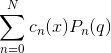
\includegraphics[width = 0.25\textwidth]{pc.png}};
%       \node[align=left] at (image2.east) {\hspace{4cm} \bf Polynomial Chaos};
%     \end{tikzpicture}

% \end{frame}




\begin{frame}{Computational models are created from experimental data}
    \begin{figure}
      \only<1>{\includegraphics[width=1\textwidth]{neuron.png}}
      \only<2->{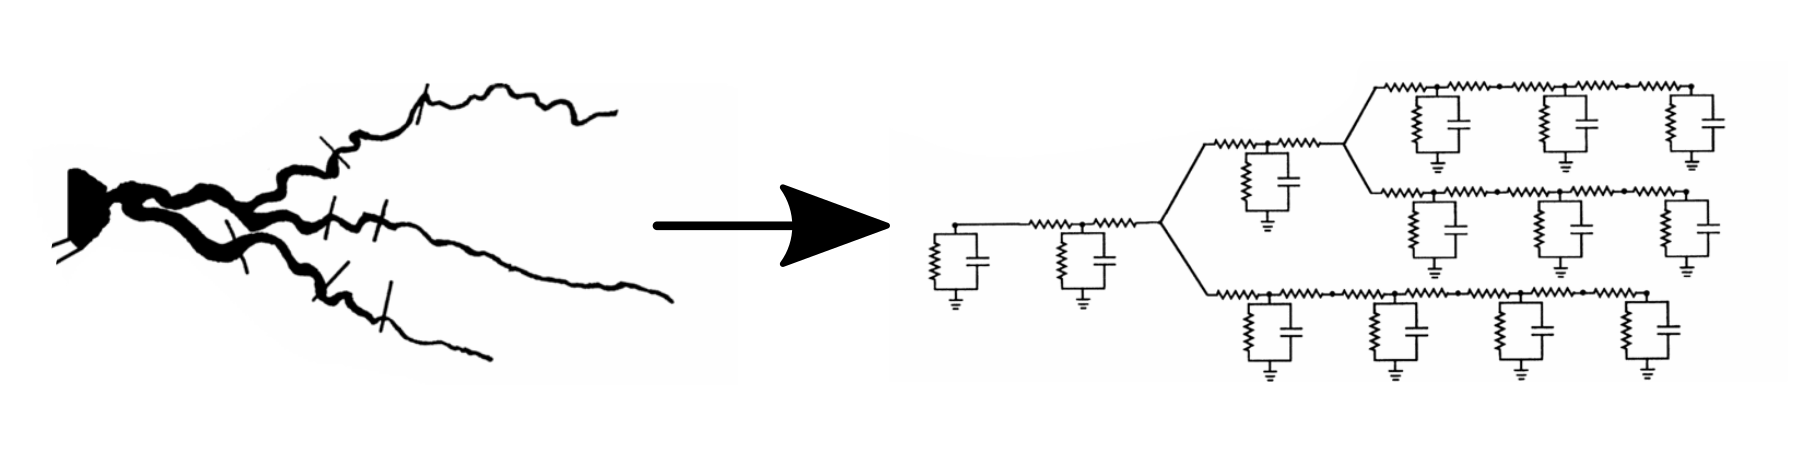
\includegraphics[width=1\textwidth]{model_creation.png}}
\end{figure}
% \vspace{5mm}
\begin{align*}
    \only<-2>{ \color{white}\frac{{\mathrm d} V_m}{{\mathrm d} }}
    \only<3>{ I &= C_m\frac{{\mathrm d} V_m}{{\mathrm d} t}  + I_{K} + I_{Na} + I_{l}}
    \only<4>{I &= C_m\frac{{\mathrm d} V_m}{{\mathrm d} t}  + {\bf\color{red}I_{K}}+ {\bf\color{red}I_{Na}} + {\bf \color{red}I_{l}}}
\end{align*}

\end{frame}


\begin{frame}{Different parameters give different model results}
    \only<1>{\[I = C_m\frac{{\mathrm d} V_m}{{\mathrm d} t}  + {\bf\color{blue}I_{K}} + {\bf\color{green}I_{Na}} + {\bf\color{red}I_{l}}\]}
    \begin{figure}
        \only<1>{
\includegraphics[width=0.4\textwidth]{parameters.png}}
        \only<2>{\includegraphics[width=1\textwidth]{hh_basic.png}}
      \end{figure}

\end{frame}



% \begin{frame}{Problem: Experimental measurements always contain errors}
%     \begin{figure}
%         \includegraphics[width=1\textwidth]{dist.png}
%     \end{figure}
% \end{frame}



\begin{frame}{Problem: Biological parameters are not fixed, but have inherent variability}
    \begin{figure}
\includegraphics[width=1\textwidth]{dist.png}
\end{figure}
\end{frame}

\begin{frame}{Solution: Perform an uncertainty quantification}
    \begin{figure}
        \includegraphics[width=0.5\textwidth]{model3.png}
    \end{figure}
\end{frame}


% \begin{frame}{Uncertainty quantification relates uncertain parameters and model results}
%     \begin{figure}
%         \only<1>{\includegraphics[width=0.5\textwidth]{model1.png}}
%         \only<2>{\includegraphics[width=0.5\textwidth]{model2.png}}
%         \only<3>{\includegraphics[width=0.5\textwidth]{model3.png}}
%         \only<4>{\includegraphics[width=0.5\textwidth]{model4.png}}
%     \end{figure}
% \end{frame}



%
% \begin{frame}{Creating a computational model consists of three steps, model creation, parameter estimation and uncertainty quantification}
%     \begin{tikzpicture}[remember picture, overlay, font=\sffamily]
%       \onslide<1-3>{\node [align=left, xshift=-0.35\textwidth,yshift=0.15\textwidth] (image3) at (current page.center)
%             {$I = C_m\frac{{\mathrm d} V_m}{{\mathrm d} t}  + I_{\text{ion channels}}$};
%       \node[align=left] at (image3.east) {\hspace{4cm} \bf Model creation};}
%     \end{tikzpicture}
%    %
%    % \begin{tikzpicture}[remember picture, overlay, font=\sffamily]
%    %   \onslide<1-3>{\node [align=left, xshift=-0.4\textwidth,yshift=0.15\textwidth] (image3) at (current page.center)
%    %         {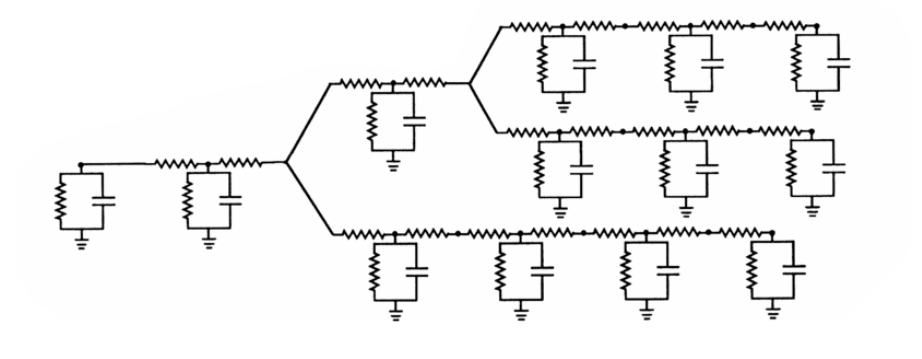
\includegraphics[width = 0.4\textwidth]{compartmental.png}};
%    %   \node[align=left] at (image3.east) {\hspace{5cm} \bf Model creation};}
%    % \end{tikzpicture}
%
%   \begin{tikzpicture}[remember picture, overlay, font=\sffamily]
%   \onslide<2-3>{\node [align=left, xshift=-0.2\textwidth,yshift=-0.05\textwidth] (image1) at (current page.center)
%       {
\includegraphics[width = 0.15\textwidth]{parameters.png}};
%   \node[align=left] at (image1.east) {\hspace{4.5cm} \bf Estimate parameters};}
%   \end{tikzpicture}
%
%     \begin{tikzpicture}[remember picture, overlay, font=\sffamily]
%       \onslide<3-4>{\node [align=left, xshift=0\textwidth,yshift=-0.25\textwidth] (image2) at (current page.center)
%             {
\includegraphics[width = 0.25\textwidth]{uq.png}};
%       \node[align=left] at (image2.east) {\hspace{4cm} \bf Quantify uncertainties};}
%     \end{tikzpicture}
%
% \end{frame}
















% \begin{frame}{Uncertainty quantification relates measurements errors and model results}
% % \begin{itemize}
% %     \item accuracy of model
% %     \item effect of uncertain input
% %     \item relationship between uncertain input and output
% %
% % \end{itemize}
% \end{frame}
\begin{frame}
    \begin{center}
        {\usebeamercolor[fg]{frametitle} \Large \bf UncertainPy performs these calculations}
    \end{center}
\end{frame}

\begin{frame}{Result: Variations in an action potential \\(90\% confidence interval)}
   \vspace{-5mm}
\begin{figure}
   \only<1>{\includegraphics[width=1\textwidth]{hh_confidence.png}}
   \only<2>{\includegraphics[width=1\textwidth]{hh_confidence_arrow.png}}
\end{figure}
\end{frame}



\begin{frame}{\onslide<1->{Point wise comparison \onslide<2->{is problematic since "the same" spike can occur at different times with different parameters}}}
   \vspace{-5mm}
   \begin{figure}
    %   \only<1>{\includegraphics[width=1\textwidth]{hh_basic.png}}
      \only<1>{\includegraphics[width=1\textwidth]{hh_line.png}}
      \only<2>{\includegraphics[width=1\textwidth]{hh_arrows.png}}
   \end{figure}
\end{frame}

% \begin{frame}{90\% confidence interval for the Hodgkin-Huxley model with original uncertainties in the parameters}
%    \vspace{-5mm}
% \begin{figure}
%    \only<1>{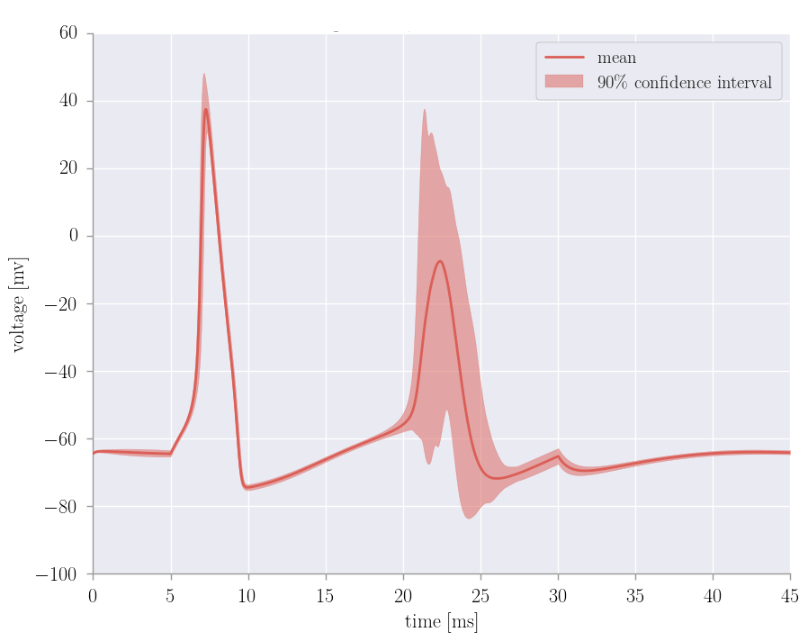
\includegraphics[width=0.8\textwidth]{confidence-interval.png}}
%    \only<2>{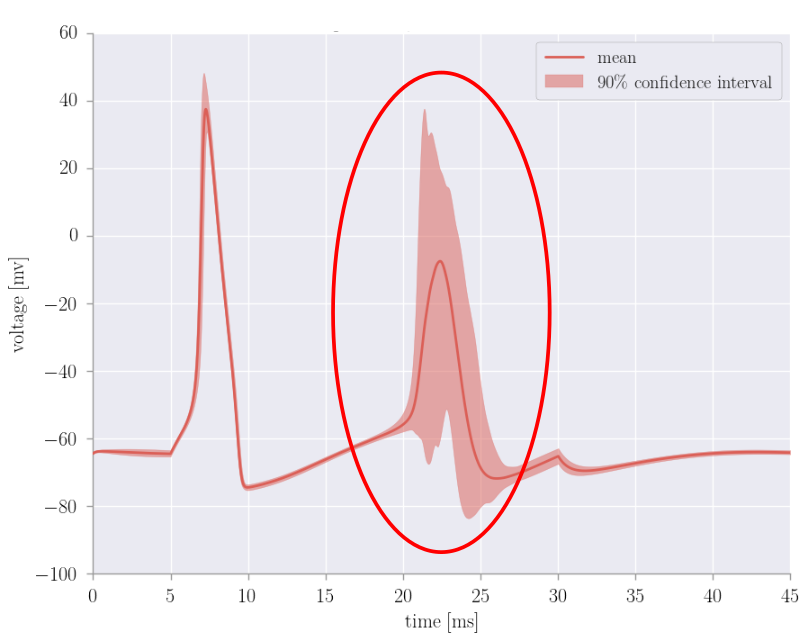
\includegraphics[width=0.8\textwidth]{confidence-interval_elipse.png}}
% \end{figure}
% \end{frame}


\begin{frame}{Solution: calculate the uncertainty for features such as the number of spikes {\color{white} dummy text dummy text dummy text dummy text dummy text} }
\vspace{-5mm}
\begin{figure}
   \includegraphics[width=1\textwidth]{hh_nrspikes.png}
\end{figure}
\end{frame}

\begin{frame}{UncertainPy calculates the uncertainty for features such as the number of spikes}
\vspace{-5mm}
\begin{figure}
   \includegraphics[width=1\textwidth]{hh_nrspikes_bar.png}
\end{figure}
\end{frame}


% \begin{frame}{Sensitivity of the result for each parameter in the Hodgkin-Huxley model}
% \vspace{-5mm}
% \begin{figure}
%    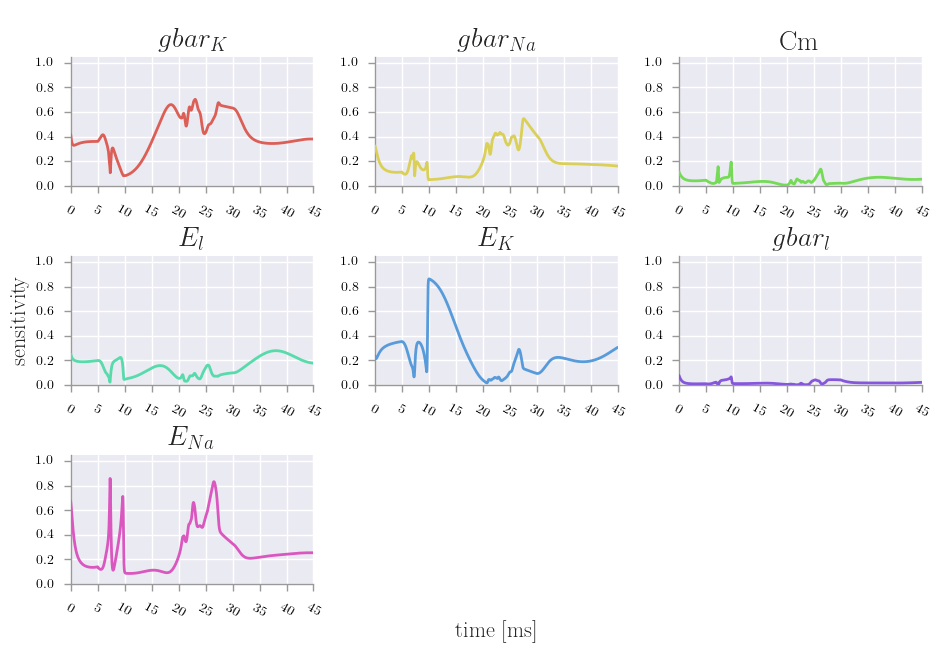
\includegraphics[width=1\textwidth]{sensitivity_grid.png}
% \end{figure}
% \end{frame}


  \begin{frame}{Summary: UncertainPy is a novel Python toolbox, tailored to perform uncertainty quantification in neuroscience models}
\vspace{-10mm}
\begin{columns}

     \column{.5\textwidth}
     \begin{center}
        \raggedright
      \bf{UncertainPy calculates uncertainties of a model from uncertain parameters}
     \end{center}
     \column{.5\textwidth}
     \begin{center}
            \includegraphics[width=0.8\textwidth]{hh_confidence_basic.png}
     \end{center}

 \end{columns}

% \vspace{5mm}

\begin{columns}
  \column{.5\textwidth}
  \begin{center}
      \raggedright
   \bf{UncertainPy is feature based}
  \end{center}
       \column{.5\textwidth}
     \begin{center}
            \includegraphics[width=0.8\textwidth]{hh_nrspikes_basic.png}
     \end{center}

 \end{columns}


   \begin{tikzpicture}[remember picture, overlay, font=\sffamily]
       \node [align=left, xshift=0.49\textwidth,yshift=-0.37\textwidth] (image2) at (current page.center)
             {
\includegraphics[width = 0.35\textwidth]{cinpla.png}};
     \end{tikzpicture}


\pause
\begin{tikzpicture}[remember picture, overlay, font=\sffamily]

  \node[align=left, yshift=0.1\textwidth] at (current page.south){ \bf \large Questions?};
\end{tikzpicture}



\end{frame}


\end{document}
